\documentclass[11pt]{article}

\usepackage{amsmath}
\usepackage{amsfonts}
\usepackage{wrapfig}
\usepackage{amssymb}
\usepackage{float}
\usepackage[dvipsnames]{xcolor}
\usepackage{graphicx}
\usepackage[siunitx, RPvoltages]{circuitikz}
\usepackage{empheq}
\usepackage{hyperref}
\usepackage{tcolorbox}
\usepackage{pgfplots}
\usepackage{caption}
\usepackage{subcaption}
\usepackage{upgreek}
\usepackage[margin=1in,headheight=13.6pt]{geometry}
\usepackage{fancyhdr}

\tcbuselibrary{breakable}
\pagestyle{fancy}
\fancyhf{}
\lhead{\fontsize{14}{15} \selectfont Time Domain Analysis}
\rfoot{Page \thepage}

\tikzset{
  declare function={% in case of CVS which switches the arguments of atan2
    atan3(\a,\b)=ifthenelse(atan2(0,1)==90, atan2(\a,\b), atan2(\b,\a));},
  kinky cross radius/.initial=+.125cm,
  @kinky cross/.initial=+, kinky crosses/.is choice,
  kinky crosses/left/.style={@kinky cross=-},kinky crosses/right/.style={@kinky cross=+},
  kinky cross/.style args={(#1)--(#2)}{
    to path={
      let \p{@kc@}=($(\tikztotarget)-(\tikztostart)$),
          \n{@kc@}={atan3(\p{@kc@})+180} in
      -- ($(intersection of \tikztostart--{\tikztotarget} and #1--#2)!%
             \pgfkeysvalueof{/tikz/kinky cross radius}!(\tikztostart)$)
      arc [ radius     =\pgfkeysvalueof{/tikz/kinky cross radius},
            start angle=\n{@kc@},
            delta angle=\pgfkeysvalueof{/tikz/@kinky cross}180 ]
      -- (\tikztotarget)}}}
\pgfplotsset{width=7cm, compat=1.16}

\counterwithin{figure}{section}
\numberwithin{equation}{section}

\newcommand*\widefbox[1]{\fbox{\hspace{2em}#1\hspace{2em}}}

\hypersetup{
	colorlinks,
	citecolor=black,
	filecolor=black,
	linkcolor=blue,
	urlcolor=cyan,
}

\title{\textbf{Time Domain Analysis}}
\author{Jay Khandkar}
\date{January 18, 2021}

\begin{document}

\begin{titlepage}
    \begin{center}
        \vspace*{1cm}
            
        \Huge
        \textbf{Time Domain Analysis}
            
        \vspace{0.5cm}
        \LARGE
        RL Circuits, RC Circuits, Sinusoidal Forcing Functions
            
        \vspace{1.5cm}
            
        \textbf{Jay Khandkar}
        \vspace{1.2cm}
            
								\begin{figure}[!h]
\centering
\begin{tikzpicture}
\begin{axis}[
	legend pos = north east,
    axis lines = left,
    yticklabels={$\frac{1}{3}V_{cc}$, $\frac{2}{3}V_{cc}$},ytick={1,2}, xtick=\empty,
    x label style = {at={(1,0)},anchor=west},
    y label style = {at={(0,1)},rotate=-90,anchor=south},
    xlabel = $t$,
    ylabel = {$v_C$}
]

\addplot [
    domain=0:2.197, 
    samples=100, 
    color=red, smooth
]
{3*(1-exp(-0.5*x))};
\addplot [
    domain=2.197:3.583, 
    samples=100, 
    color=red, smooth
]
{2*exp(-0.5*(x-2.197))};
\addplot [
    domain=3.583:4.969, 
    samples=100, 
    color=red, smooth
]
{3*(1-exp(-0.5*(x-2.772)))};
\addplot [
    domain=4.969:6.357, 
    samples=100, 
    color=red, smooth
]
{2*exp(-0.5*(x-4.969))};
\addplot [
    domain=6.357:7.740, 
    samples=100, 
    color=red, smooth
]
{3*(1-exp(-0.5*(x-5.544)))};



\end{axis}
\end{tikzpicture}
\caption*{\textit{The astable 555 timer IC waveform}}
\end{figure}   
        
            
        \vspace{0.8cm}
           
            
        \Large
        January 18, 2021
        
            
    \end{center}
\end{titlepage}

\newpage
\tableofcontents
\newpage
\begin{flushleft}
\color{blue}
\section{Current And Voltage Conventions}
\color{black}

The conventions we shall follow, called \textit{\textbf{passive sign conventions}}, simply state that when 
current ``flows into" the positive terminal of the capacitor/inductor, as indicated by the polarity of $v$
in Fig.\ref{fig:conventions}, it is taken as positive. We may then write the current-voltage relations:

\begin{empheq}[box=\widefbox]{align*}
i &= C\frac{dv}{dt}\\
v &= L\frac{di}{dt}
\end{empheq}

\begin{figure}[H]
\centering
\fbox{
\begin{circuitikz}[american]
	
	\draw (0,0) to[short, i=$i$] (1,0) to[C, l=$C$, v_=$v$, o-o, voltage shift=2.5] (2,0) 
	to[short] (3,0);
	\draw (0,-2) to[short, i=$i$] (1,-2) to[cute inductor, l=$L$, v^=$v$, o-o, voltage shift=5.0] (2,-2) 		to[short] (3,-2);
	
\end{circuitikz}
}
\caption{The voltage conventions}
\label{fig:conventions}	
\end{figure}

\color{blue}
\section{First Order Circuits: RL and RC}
\color{black}
A first order circuit is one that is governed by a first order differential equation. Often, it is
incorrectly stated that a first order circuit is one that contains only one energy storage element
(capacitor/inductor). This is wrong, as there are certain arrangements of $R-L$ and $R-C$ circuits
which can be simplified to obtain a first order equation, as we shall see later. So, there being only
one energy storage element in a circuit is a \textit{sufficient} but not \textit{necessary} condition for
it to be first order.

\color{blue}
\subsection{The Natural Response}
\subsubsection{The Source-Free RL Circuit}
\color{black}
A \textbf{\textit{natural response}} is one that is free of any external voltage/current sources, 
which are also known as \textit{forcing functions}. It depends on the ``general nature" of the circuit
(types of elements, sizes and interconnections). It is also known as the \textbf{\textit{transient
response}}, as without any external sources, it must eventually die out. Consider the simple series RL
circuit shown in Fig.\ref{fig:src_free_RL}:
\newpage
\begin{figure}[!h]
\centering
\begin{circuitikz}[american]
	\draw (0,0) to [R=$R$, v>=$v_R$, voltage shift=2.5] (0,3) to [short, i=$i(t)$] (3,3)
			to [cute inductor, l=$L$, v=$v_L$] (3,0) to [short] (0,0); 
\end{circuitikz}
\caption{Simple R-L circuit for which $i(t)$ is to be determined}
\label{fig:src_free_RL}	
\end{figure}

Let the time varying current be designated $i(t)$, and the value of $i$ at $t=0$ be $I_0$. It may seem 
counter-intuitive to have a non-zero current initially in a circuit with no sources. In order 
for a current to be flowing, a source had to be present at some point of time, but we are only 
bothered with the response of the circuit after $t=0$, 
ie. after the source has been removed. Applying Kirchhoff's
voltage law, we have
\begin{equation*}
Ri + v_L = Ri + L\frac{di}{dt} = 0 
\end{equation*}
or
\begin{equation}
\label{equation:rl_natural}
\frac{di}{dt} + \frac{R}{L}i = 0
\end{equation}
We can separate variables and integrate easily, giving

\begin{equation}
\label{equation:rl_nat_resp}
\boxed{i(t) = I_0e^{-\frac{R}{L}t}}
\end{equation}

where we have incorporated the intitial codition $i(0)=I_0$. The general form of the natural response will 
be
\begin{equation}
\boxed{i(t) = Ke^{-\frac{R}{L}t}}
\end{equation}
where $K$ is a constant, and is nothing but the value of $i$ at $t=0$.

\paragraph{\color{blue}Accounting For The Energy}\mbox{} \\ \mbox{}\\
The power dissipated through the resistor at any time $t$

\begin{equation*}
p_R = i^{2}R = I_0^{2}Re^{-\frac{2Rt}{L}}
\end{equation*}

and the total energy turned into heat by the resistor till the response has died out

\begin{align*}
w_R &= \int_{0}^{\infty} p_R\,dt\\
    &= I_0^{2}R\int_{0}^{\infty} e^{-\frac{2Rt}{L}}\,dt\\
    &= I_0^{2}R\left (\frac{-L}{2R}\right)e^{-\frac{2Rt}{L}}\Biggr|_{0}^{\infty}\\
\Aboxed{w_R &= \frac{1}{2}LI_0^{2}}
\end{align*}
which is the total energy stored initially in the inductor, as expected.

\color{blue}
\subsubsection{Properties Of The Natural Response}
\color{black}

\begin{figure}[H]
\centering
\begin{tcolorbox}[colframe=black, hbox]
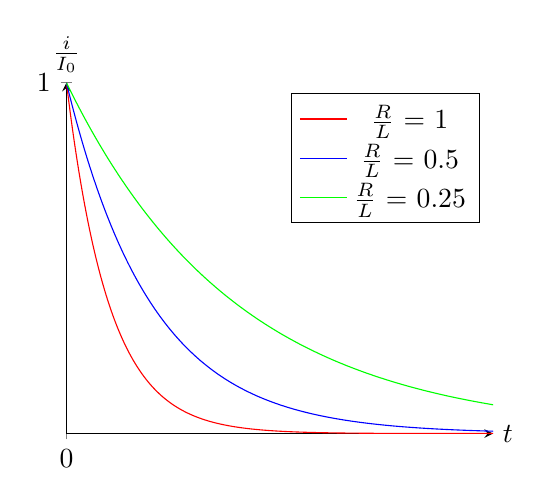
\begin{tikzpicture}
\begin{axis}[
	legend pos = north east,
    axis lines = left,
    ytick={1}, xtick={0},
    x label style = {at={(1,0)},anchor=west},
    y label style = {at={(0,1)},rotate=-90,anchor=south},
    xlabel = $t$,
    ylabel = {$\frac{i}{I_0}$},
]

\addplot [
    domain=0:10, 
    samples=100, 
    color=red, smooth
]
{exp(-x)};
\addlegendentry{$\frac{R}{L}$ = 1}
\addplot [
    domain=0:10, 
    samples=100, 
    color=blue, smooth
]
{exp(-0.5*x)};
\addlegendentry{$\frac{R}{L}$ = 0.5}
\addplot [
    domain=0:10, 
    samples=100, 
    color=green, smooth
]
{exp(-0.25*x)};
\addlegendentry{$\frac{R}{L}$ = 0.25}

\end{axis}
\end{tikzpicture}
\end{tcolorbox}
\caption{Some possible plots for the natural response}
\label{fig:nat_resp}
\end{figure}


From the natural response of the series RL circuit given by Eq.\ref{equation:rl_nat_resp}, it is clear that
that the current decays exponentially to zero from an initial value of $I_0$. The graph of $\frac{i}{I_0}$
is plotted in figure \ref{fig:nat_resp} for three different values of $\frac{R}{L}$, as indicated in the legend.

Consider now the initial rate of decay, which is found by differentiating equation \ref{equation:rl_nat_resp}:

\begin{equation*}
\frac{d}{dt}\frac{i}{I_0}\Biggr|_{t=0} = -\frac{R}{L}e^{-Rt/L}\Biggr|_{t=0} = -\frac{R}{L}
\end{equation*}
Assuming that the decay continues at this rate, the time $\uptau$ taken by $\frac{i}{I_0}$ to drop from
$1$ to $0$ is given by
\begin{equation*}
\left(\frac{R}{L}\right)\uptau = 1
\end{equation*}
or
\begin{equation}
\boxed{\uptau = \frac{L}{R}}
\end{equation}
The constant $\uptau$ has the units of seconds and is called the \textbf{time constant} of the circuit.
It may be found graphically from the response curve by drawing the tangent to the curve at $t=0$ and
finding where it intersects the $x$ axis, as shown below:


\begin{figure}[H]
\centering
\begin{tcolorbox}[colframe=black, hbox]
\begin{tikzpicture}
\begin{axis}[
	ytick={1}, xtick={0,2},
	x label style = {at={(1,0)},anchor=west},
	y label style = {at={(0,1)},rotate=-90,anchor=south},
    axis lines = left,
    xlabel = $t$,
    ylabel = {$\frac{i}{I_0}$},
    ymin = 0, ymax = 1
]

\addplot [
    domain=0:10, 
    samples=100, 
    color=red, smooth
]
{exp(-0.5*x)};
\addplot [
	domain=0:10,
	color=blue, smooth
]
{-0.5*x+1};
\addplot[mark=*] coordinates {(2,0)} node[pin=150:{$\uptau$}]{} ;

\end{axis}
\end{tikzpicture}
\label{fig:finding_tau_graphically}
\end{tcolorbox}
\caption{Finding the time constant graphically}
\end{figure}


Yet another way to define the time constant is to note that
\begin{equation*}
\frac{i(\uptau)}{I_0} = e^{-1} = 0.3679
\end{equation*}
ie, in one time constant, the response falls to $36.8\%$ of it's initial value. The value of $\uptau$ may
also be determined from this fact:


\begin{figure}[H]
\centering
\begin{tcolorbox}[colframe=black, hbox]
\begin{tikzpicture}
\begin{axis}[
	ytick={0.1353,0.3679,1}, xticklabels={0, $\uptau$, $2\uptau$},xtick={0,2,4},
	x label style = {at={(1,0)},anchor=west},
	y label style = {at={(0,1)}, rotate=-90, anchor=south},
    axis lines = left,
    xlabel = $t$,
    ylabel = {$\frac{i}{I_0}$},
    ymin = 0, ymax = 1
]

\addplot [
    domain=0:10, 
    samples=100, 
    color=red, smooth
]
{exp(-0.5*x)};
\addplot[mark=none, black, dashed] coordinates {(0, 0.3679) (2, 0.3679)};
\addplot[mark=none, black, dashed] coordinates {(2, 0.3679) (2, 0)};

\addplot[mark=none, black, dashed] coordinates {(0, 0.1353) (4, 0.1353)};
\addplot[mark=none, black, dashed] coordinates {(4, 0.1353) (4, 0)};

\end{axis}
\end{tikzpicture}
\label{fig:finding_tau_graphically_2}
\end{tcolorbox}
\end{figure}


\begin{tcolorbox}[colback=blue!5, colframe=blue!75!black, title=\textbf{Example 2.1}, breakable]
\begin{figure}[H]
\centering
\begin{circuitikz}[american, scale=0.9, transform shape]
	\draw (0,0) to [R=40<\Omega>, v>=$v$, voltage shift=2.5] (0,4) to [short, -*] (2,4)
				to [opening switch,l=${t=0s}$, o-o] (2,2) to [american voltage source, 
				v=24<\volt>, o-o, invert] (2,0); 
	\draw  (2,4) to [R=10<\Omega>] (5,4) to [cute inductor, l=5<\henry>,i=$i_L$] (5,0) to 
			[short] (0,0);
\end{circuitikz}
\caption{A simple RL circuit with a switch thrown at $t=0$}
\label{fig:example_circuit}	
\end{figure}

For the circuit given in figure \ref{fig:example_circuit}, let us try to find the voltage at 
$t=200ms$.\\~\\

Figures \ref{fig:prior_t_0} and \ref{fig:post_t_0} show the state of the circuit prior to and post the 
throwing of the switch. In \ref{fig:prior_t_0}, the inductor acts like a short to DC current after all transients have died down.

\begin{figure}[H]
\centering
\begin{subfigure}{.5\textwidth}
  \centering

  \begin{circuitikz}[american, scale=0.9, transform shape]
	\draw (0,0) to [R=40<\Omega>, v>=$v$, voltage shift=2.5] (0,4) to [short, -*] (2,4)
				to [american voltage source, v=24<\volt>, o-o, invert] (2,0); 
	\draw  (2,4) to [R=10<\Omega>] (5,4) to [short, i=$i_L$] (5,0) to 
			[short] (0,0);
  \end{circuitikz}
  
  \caption{The circuit prior to $t=0$}
  \label{fig:prior_t_0}
\end{subfigure}%
\begin{subfigure}{.5\textwidth}
  \centering
  
  \begin{circuitikz}[american, scale=0.9, transform shape]
	\draw  (0,0) to [R=40<\Omega>, v>=$v$, voltage shift=2.5] (0,4) to [R=10<\Omega>] (5,4) to 
				[cute inductor,l=5<\henry>,i=$i_L$] (5,0) to [short] (0,0);
  \end{circuitikz}
  
  \caption{The circuit post $t=0$}
  \label{fig:post_t_0}
\end{subfigure}
\caption{The simplified circuit before and after the switch is opened}
\label{fig:example_1}
\end{figure}


Applying Kirchhoff's Law in \ref{fig:post_t_0}, we may write 

\begin{align*}
-v + 10i_L + 5\frac{di_l}{dt} &= 0\\
\Rightarrow \frac{5}{40}\frac{dv}{dt} + \left(\frac{10}{40}+1\right)v &= 0\\
\Rightarrow \frac{dv}{dt} + 10v &= 0
\end{align*}
where we have taken $i_l = -v/40$ by our conventions. The solution to this differential equation is
\begin{equation*}
v(t) = v(0^{+})e^{-10t}
\end{equation*}
%\end{tcolorbox}

%\begin{tcolorbox}[colback=red!5, colframe=red!75!black]
Note that the initial value of voltage here is denoted by $v(0^{+})$, as the voltage across the resistor 
may change discontinuously when the switch is thrown. We have to use the fact that $i_L$ cannot 
change discontinuously, and remains the same just before and just after the switch is 
thrown. From \ref{fig:prior_t_0}, $i_l(0) = 24/10 = 2.4\text{A}$. Hence, $v(0^{+}) = (40)\cdot(-2.4)=-96\text{V}$, and
so
\begin{equation*}
\boxed{v(t) = -96e^{-10t}}
\end{equation*}
which gives $v(0.2) = -12.99\text{V}$.
\end{tcolorbox}
%{\color{red} \rule{\linewidth}{0.5mm}}

\color{blue}
\subsubsection{The Source-Free RC Circuit}
\color{black}

\begin{figure}[!h]
\centering
\begin{circuitikz}[american]
	\draw (0,0) to [R=$R$, v>=$v_R$, voltage shift=2.5] (0,3) to [short, i=$i(t)$] (3,3)
			to [C, l=$C$, v=$v_C$, voltage shift=1.5] (3,0) to [short] (0,0); 
\end{circuitikz}
\caption{Source-Free RC Circuit}
\label{fig:src_free_RC}	
\end{figure}
The source free response for RC circuits is nearly the same as with LC, but with slightly different 
expressions for the time constant. In this case, the general form of the response is given by

\begin{equation}
\boxed{v(t) = v(0)e^{-\frac{t}{\uptau}}}
\end{equation}

and the expression for the time constant is

\begin{equation}
\boxed{\uptau = R \cdot C}
\end{equation}

It may also be noted that the voltage across a capacitor cannot change discontinuously, as opposed to
the current for an inductor.

\color{blue}
\subsubsection{General RL and RC Circuits}
\color{black}

For circuits containing more than one capacitor/inductor and more than one resistor, it is possible
to arrive at a single time constant and reduce it to a simple circuit with one resistor and one
energy storage element, as long as the Th\'{e}venin resistance ``seen" by all the elements is the same.
In such a case, we can write $\uptau = \frac{L_{eq}}{R_{eq}}$ or $\uptau = R_{eq} \cdot C_{eq}$.
The general form of the natural response would then be $Ae^{-t/\uptau}$, where the constant A 
can be determined using the initial conditions, and would be different for different elements.
Let us illustrate this using the following example:\\~\\

\begin{tcolorbox}[colback=blue!5, colframe=blue!75!black, title=\textbf{Example 2.2}, breakable]
\begin{figure}[H]
\centering
\begin{subfigure}{.5\textwidth}
  \centering
  
  \begin{circuitikz}[american, scale=0.6, transform shape]
	\draw (0,0) -- (0,5) to [R=120<\Omega>] (4,5) to [R=60<\Omega>] (4,3) to [cute inductor,
		l=1<\milli\henry>, i=$i_L$] (8,3) to [R=50<\Omega>] (9,3) to [short, -*] (10,3)to[cute inductor,
		l=2<\milli\henry>] (10,0)to [short, -*](10,0) to [short] (0,0);
	\draw (10,3) -- (12,3) to [cute inductor, l=3<\milli\henry>] (12,0) to [short, -*] (4,0)
		to [R, l_=$90\Omega$,i_<=$i_1$] (4,3) to [short, -*] (4,3) to [opening switch,l=${t=0s}$, *-*] (2,3)
		to [american voltage source, v=18<\volt>, *-*, invert] (2,0);
  \end{circuitikz}
  
  \caption{The circuit with multiple inductors and resistors}
  \label{fig:example_circ_2}
\end{subfigure}%
\begin{subfigure}{.5\textwidth}
  \centering
  
 \begin{circuitikz}[american, scale=0.6, transform shape]
	\draw (0,0) -- (0,5) to [R=120<\Omega>] (2,5) to [R=60<\Omega>] (2,3) to [cute inductor,
		l=1<\milli\henry>, i=$i_L$] (6,3) to [R=50<\Omega>] (7,3) to [short, -*] (8,3)to[cute inductor,
		l=2<\milli\henry>] (8,0)to [short, -*](8,0) to [short] (0,0);
	\draw (8,3) -- (10,3) to [cute inductor, l=3<\milli\henry>] (10,0) to [short, -*] (2,0)
		to [R, l_=$90\Omega$,i<=$i_1$] (2,3)to [short, -*] (2,3);
  \end{circuitikz}
  
  \caption{The simplified circuit after $t=0$}
  \label{fig:simplified_circ_2}
\end{subfigure}
\label{fig:example_2}
\end{figure}

For the circuit given in figure \ref{fig:example_circ_2} find $i_1$ and $i_L$ for 
$t>0$.\\~\\


Firstly, note that the equivalent/Th\'{e}venin resistance seen by all three inductances is equal, and equal
to $50 + 90||(120 + 60) =110\Omega$. So, we can reduce it to a simple LR circuit, with

\begin{align*}
L_{eq} &= \frac{2 \cdot 3}{2+3} + 1 = 2.2 mH\\
\Rightarrow \uptau &= \frac{L_{eq}}{R_{eq}} = 20\mu s 
\end{align*}
And so every current and voltage in the network must have the form $Ke^{-t/\uptau}=Ke^{-50,000t}$.
If we consider the circuit prior to opening the switch and after all transients have died down, the
inductors act as shorts to DC current and so $i_L$ is easily found to be $i_L = 18/50 = 360mA$. This must
also be the value of $i_L$ just after the switch is opened. So,

\begin{equation*}
i_L = \begin{cases} 
          360 mA & t < 0 \\
          360e^{-50,000t} mA & 0\leq t 
       \end{cases}
\end{equation*}

Now, $i_1$ may change discontiuously at $t=0$ so we have to find it's value at $0^{+}$ using the value of
$i_L(0^+)$. Using current division,

\begin{equation*}
i_1(0^+) = -i_L(0^+) \cdot \frac{120+60}{120+60+90} = -240 mA
\end{equation*}

Hence,

\begin{equation*}
i_1 = \begin{cases} 
          200 mA & t < 0 \\
          -240e^{-50,000t} mA & 0\leq t 
       \end{cases}
\end{equation*}
\end{tcolorbox}

\color{blue}
\subsection{The Unit Step Function}
\color{black}
The unit step function, also called the \href{https://en.wikipedia.org/wiki/Oliver_Heaviside}
{\textbf{Heaviside step function}} is a step function whose value is zero for negative arguments and
one for positive arguments. This function is important as the switching action of a battery is equivalent
to a forcing function which is zero up until the switch is thrown, and equal to the battery voltage
thereafter. It is represented by $u$, $\theta$ or $H$.\\
If we shift the argument to some arbitrary time $t_0$, then $u(t-t_0)$ must be zero for all values of $t$
less than $t_0$ and unity for values of $t$ greater than $t_0$. The unit step function changes abruptly/
discontinuously from $0$ to $1$, and it's value at $t=t_0$ is not defined.\\
It can be represented analytically as

\begin{equation*}
u(t-t_0) = \begin{cases} 
          0 & t < t_0 \\
          1  & t > t_0 
       \end{cases}
\end{equation*}

or graphically as\\~\\

\begin{tcolorbox}[colframe=black]
\begin{figure}[H]
\centering
\begin{subfigure}{.5\textwidth}
	\centering
  \begin{tikzpicture}
	\begin{axis}[
        axis lines = middle,
		ytick={1}, xticklabels={0, $t_0$},xtick={0,2},
		x label style = {at={(axis description cs:1,0.111)},anchor=west},
		y label style = {at={(axis description cs:0.090,1)},anchor=south},
    	xlabel = $t$,
    	ylabel = {$u(t-t_0)$},
   	 ymin = -0.25, ymax = 2,
   	 xmin=-0.5, xmax=5
	]

	\addplot [
    	domain=-1:2, 
    	samples=100, 
    	color=red, smooth, ultra thick
	]
	{0};
	\addplot [
    	domain=2:5, 
    	samples=100, 
    	color=red, smooth, ultra thick
	]
	{1};
	\addplot[mark=none, red, ultra thick] coordinates {(2,0) (2, 1)};
	%following code is just a way to label zero for middle axis
	\node[
    anchor=north east,
    outer sep=.5*\pgflinewidth+.5*\pgfkeysvalueof{/pgfplots/major tick length},
    %draw,green% to show the border of the node
    ]
    at({xticklabel* cs:0}-|{yticklabel* cs:0})
    {\pgfmathprintnumber{0}};
	\end{axis}
	\end{tikzpicture}
  
  \label{fig:unit_step_1}
\end{subfigure}%
\begin{subfigure}{.5\textwidth}
	\centering
  \begin{tikzpicture}
	\begin{axis}[
        axis lines = middle,
		ytick={0,1}, xtick={0},
		x label style = {at={(axis description cs:1,0.111)},anchor=west},
		y label style = {at={(axis description cs:0.222,1)},anchor=south},
    	xlabel = $t$,
    	ylabel = {$u(t)$},
   	 ymin = -0.25, ymax = 2,
   	 xmin=-2, xmax=7
	]

	\addplot [
    	domain=-2:0, 
    	samples=100, 
    	color=red, smooth, ultra thick
	]
	{0};
	\addplot [
    	domain=0:7, 
    	samples=100, 
    	color=red, smooth,ultra thick
	]
	{1};
	\node[
    anchor=north east,
    outer sep=.5*\pgflinewidth+.5*\pgfkeysvalueof{/pgfplots/major tick length},
    %draw,green% to show the border of the node
    ]
    at({xticklabel* cs:0}-|{yticklabel* cs:0})
    {\pgfmathprintnumber{0}};
	\addplot[mark=none, red, ultra thick] coordinates {(0,0) (0, 1)};
	\end{axis}
	\end{tikzpicture}
  \label{fig:unit_step_2}
\end{subfigure}
\caption{The unit step function}
\label{fig:unit_step}
\end{figure}
\end{tcolorbox}

Note that the vertical line is not really a part of the unit step's definition but it is usally shown in
each drawing as it looks nicer.\\~\\

\begin{figure}[H]
\centering
\begin{subfigure}{.33\textwidth}
	\centering
  	\begin{circuitikz}[american]
	\draw (0,0) to [american voltage source, l=$5u(t-2)V$] (0,3) -- (1,3);
	\draw (0,0) -- (1,0);
	\filldraw [fill=blue!20!white, draw=blue!20!black] (1,-0.25) rectangle (3,3.25); 
	\draw (2,1.5) node [align=center] {General\\ Network};
  \end{circuitikz}
  \caption{}
  \label{fig:voltage_step}
\end{subfigure}%
\begin{subfigure}{.33\textwidth}
	\centering
	\begin{circuitikz}[american]
	\draw (0,0) to [american voltage source, v=5<\volt>](0,2)to[closing switch, l=${t=2s}$] (0,3) -- (1,3);
	\draw (0,0) -- (1,0);
	\filldraw [fill=blue!20!white, draw=blue!20!black] (1,-0.25) rectangle (3,3.25); 
	\draw (2,1.5) node [align=center] {General\\ Network};
  \end{circuitikz}
  \caption{}
  \label{fig:wrong_eq}
\end{subfigure}
\begin{subfigure}{.33\textwidth}
	\centering
	\begin{circuitikz}[american]
	\draw (0,2.65) node[cute spdt up arrow, rotate=90](Sw){};
	\draw (0,0) to [american voltage source, v=5<\volt>] (Sw.in);
	%\draw (0,0) -- (1,0);
	\filldraw [fill=blue!20!white, draw=blue!20!black] (1,-0.25) rectangle (3,3.25); 
	\draw (2,1.5) node [align=center] {General\\ Network};
	\draw (Sw.out 2) -- +(0.55,0);
	\draw (Sw.out 1) -- ++(-1.0, 0) -- ++(0,-3.03) -- +(2.40,0);
	\draw (Sw.out 2) node [align=center, anchor=south] {\small $t=2s$};
  \end{circuitikz}
  \caption{}
  \label{fig:right_eq}
\end{subfigure}
\caption{(a) The voltage-step forcing function. (b) A possible equivalent. (c) The exact equivalent.}
\label{fig:unit_physical_equiv}
\end{figure}

Interestingly, the physical equivalent of the unit step is not actually a simple voltage source in series
with a switch. Consider the step voltage source shown in figure  \ref{fig:voltage_step}. Let us try to draw it's physical 
equivalent. On first thought, one might come up with figure \ref{fig:wrong_eq}. However, these two circuits are not
equivalent for $t<2s$: the voltage across the network in figure  \ref{fig:wrong_eq} is completely unspecified in this time interval. The actual equivalent to the step voltage source is the single-pole double throw switch shown in
figure \ref{fig:right_eq}. Clearly, the voltage is zero for $t<2s$, and this is consistent with the step voltage function.

\color{blue}
\subsubsection{The Rectangular Pulse Function}
\color{black}

Various rectangular pulses may be obtained by manipulating the unit step function. Let us first consider
the pulse given by

\begin{equation*}
v(t) = \begin{cases} 
          0 & t < t_0 \\
          V_0  & t_0 < t < t_1\\
          0 & t > t_1 
       \end{cases}
\end{equation*}
Let us try to break this down into individual unit step functions. Figure \ref{fig:superposition_unit_steps} shows the superposition of the two step functions $u(t-t_0)$ and 
$-u(t-t_1).$ Clearly, their superposition gives the rectangular pulse in figure \ref{fig:rect_pulse_}. \\~\\

\begin{tcolorbox}[colframe=black]
\begin{figure}[H]
\centering
\begin{subfigure}{.5\textwidth}
	\centering
  \begin{tikzpicture}
	\begin{axis}[
        axis lines = middle,
		ytick={1}, xticklabels={0, $t_0$, $t_1$},xtick={0,2,3},
		x label style = {at={(axis description cs:1,0.111)},anchor=west},
		y label style = {at={(axis description cs:0.0909,1)},anchor=south},
    	xlabel = $t$,
    	ylabel = {$v(t)$},
   	 ymin = -0.25, ymax = 2,
   	 xmin=-0.5, xmax=5
	]

	\addplot [
    	domain=-1:2, 
    	samples=100, 
    	color=red, smooth, ultra thick
	]
	{0};
	\addplot [
    	domain=2:3, 
    	samples=100, 
    	color=red, smooth, ultra thick
	]
	{1};
	\addplot [
    	domain=3:5, 
    	samples=100, 
    	color=red, smooth, ultra thick
	]
	{0};
	\addplot[mark=none, red, ultra thick] coordinates {(2,0) (2, 1)};
	\addplot[mark=none, red, ultra thick] coordinates {(3,1) (3, 0)};
	%following code is just a way to label zero for middle axis
	\node[
    anchor=north east,
    outer sep=.5*\pgflinewidth+.5*\pgfkeysvalueof{/pgfplots/major tick length},
    %draw,green% to show the border of the node
    ]
    at({xticklabel* cs:0}-|{yticklabel* cs:0})
    {\pgfmathprintnumber{0}};
	\end{axis}
	\end{tikzpicture}
  \caption{The Rectangular Pulse}
  \label{fig:rect_pulse_}
\end{subfigure}%
\begin{subfigure}{.5\textwidth}
	\centering
  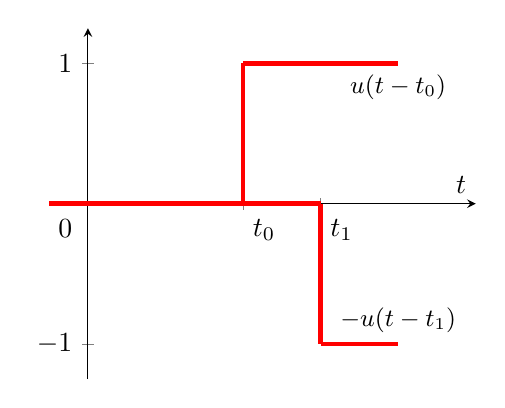
\begin{tikzpicture}
	\begin{axis}[
		ytick={-1,0,1}, xtick={0,2,3}, xticklabel style={anchor=north west}, xticklabels={0, $t_0$,$t_1$},
		x label style = {at={(5,0)},anchor=west},
		y label style = {at={(0,1.25)},rotate=-90,anchor=south},
   		 axis lines = middle,
    	xlabel = $t$,
   	 ymin = -1.25, ymax = 1.25,
   	 xmin=-0.5, xmax=5
	]

	\addplot [
    	domain=-0.5:3, 
    	samples=100, 
    	color=red, smooth, ultra thick
	]
	{0};
	\addplot [
    	domain=2:4, 
    	samples=100, 
    	color=red, smooth,ultra thick
	]
	{1} node [below, pos=1, color=black] {\small $u(t-t_0)$ };
	\addplot [
    	domain=3:4, 
    	samples=100, 
    	color=red, smooth,ultra thick
	]
	{-1} node [above, pos=1, color=black] {\small $-u(t-t_1)$};
	\node[
    anchor=north east,
    outer sep=.5*\pgflinewidth+.5*\pgfkeysvalueof{/pgfplots/major tick length},
    %draw,green% to show the border of the node
    ]
    at({xticklabel* cs:0}-|{yticklabel* cs:0})
    {\pgfmathprintnumber{0}};
	\addplot[mark=none, red, ultra thick] coordinates {(2,0) (2, 1)};
	\addplot[mark=none, red, ultra thick] coordinates {(3,0) (3, -1)};
	\end{axis}
	\end{tikzpicture}
    \caption{Superposition of two unit step functions}
    \label{fig:superposition_unit_steps}
\end{subfigure}
\label{fig:rect_pulse}
\end{figure}
\end{tcolorbox}

Breaking down rectangular pulses in terms of unit step functions can be quite handy for linear networks, for which we can simply consider individual
unit step sources separately and add them to get the total response.

\color{blue}
\subsection{The Forced Response}
\color{black}

Let us now subject a simple network to the sudden application of a DC source. Figure \ref{fig:driven_rl} shows a circuit for which $i(t)$ is to be
determined,
consisting of a voltage source in series with a resistance and an inductor, with the switch thrown at $t=0s$. Note that we also could have removed the switch and represented the voltage source as $V_0u(t)$ (not \textit{exactly} correct, as said previously).

\begin{figure}[H]
    \centering
    \begin{circuitikz}[american]
        \draw (0,0) to [american voltage source, l=$V_0$] (0,3) to [closing switch, l=${t=0s}$] (2,3) to [R=$R$, i=$i(t)$] (4.5,3)
                to [cute inductor, l=$L$] (4.5,0) --(0,0);
    \end{circuitikz}
    \caption{The Driven RL Circuit}
    \label{fig:driven_rl}
\end{figure}

Clearly, $i(t)=0$ for $t<0s$. For $t>0s$, we may apply Kirchhoff's voltage law and obtain the differential equation

\begin{equation}
 Ri + L\frac{di}{dt} = V_0
\end{equation}

Now, we can separate variables and integrate easily:

\begin{align*}
 \int_{0}^{i} \frac{L}{V_0-Ri}\,di &= \int_{0}^{t} dt\\
 \Rightarrow \frac{L}{R}\ln (V_0-Ri)\Biggr|_{0}^{i} &= t\\
 \Rightarrow i(t) &= \frac{V_0}{R}(1-e^{-Rt/L})
\end{align*}

 which is the response for $t>0s$. Note that here $i(0^-)=i(0^+)=0$. The complete response may be written conveniently in terms of the unit
 step function as 
 
 \begin{equation}
  \boxed{i(t) = \frac{V_0}{R}(1-e^{-Rt/L})u(t)} \label{equation:rl_driven}
 \end{equation}

We have arrived at this expression purely by mathematical methods. There is an easier way to arrive at this expression, and it's convenience
is highlighted even more when analysing second order driven circuits. For now, let us try to interpret the terms appearing in equation
\ref{equation:rl_driven}.\\~\\
There is one constant, $\frac{V_0}{R}$ and our familiar expression for natural circuits: $\frac{V_0}{R}e^{-t/\uptau}$. The constant is nothing
but the current at steady state, after transients have died down and is also called the \textit{steady state response, particular solution} or the
\textit{particular integral}. It is found simply by analysing the circuit at steady state - shorting all inductors and opening all capacitors.\\
The other term is the natural response, which approaches zero as the time increases without limit. The amplitude of this natural response
will depend on the initial value of the complete response, and hence also on the initial value of the forcing function. Let us now try
arriving at equation \ref{equation:rl_driven} in this new light. The total response will comprise of a natural response, $i_n$ and a forced
response, $i_f$. Hence, 

\begin{equation*}
i = i_n + i_f
\end{equation*}

where $i_n$ must have the form $Ae^{-Rt/L}$, where $A$ is a constant to be determined using the initial condition of the forcing function. The value
of $i_f$ is found by considering the circuit after the natural response has died out, when the inductor will act as a short. Clearly, in this 
condition, we have a single resistor in series with the voltage source and hence $i_f = \frac{V_0}{R}$. So,

\begin{equation*}
i = \frac{V_0}{R} + Ae^{-Rt/L}
\end{equation*}

We may now apply the initial condition $i(0^-)=i(0^+)=0$:

\begin{align*}
0 &= \frac{V_0}{R} + Ae^{0}\\
\Rightarrow A &= -\frac{V_0}{R}
\end{align*}
 
 and so we have 
 
\begin{equation*}
i(t) = \frac{V_0}{R}(1-e^{-Rt/L})u(t)
\end{equation*}
 
 The response is plotted in figure \ref{fig:forced_RC_plot}, and it is clear how $i$ rises from it's intial value of $0$ to it's forced value of $\frac{V_0}{R}$. In this 
 case, a tangent drawn to the response curve at $t=0$ meets the forced response at $t=\uptau$.\\~\\
 \begin{tcolorbox}
 \begin{figure}[H]
	\centering
  \begin{tikzpicture}
	\begin{axis}[
        axis lines = middle,
		yticklabels= {$0.632V_0/R$, $V_0/R$}, ytick = {0.632*2,2}, xticklabels={0, $\uptau$,$2\uptau$,$3\uptau$},xtick={0,1,2,3},
		x label style = {at={(axis description cs:1,0.117)},anchor=west},
		y label style = {at={(axis description cs:0.0909,1)},anchor=south},
    	xlabel = $t$,
    	ylabel = {$i(t)$},
   	 ymin = -0.4, ymax = 3,
   	 xmin=-0.5, xmax=5
	]

	\addplot [
    	domain=0:5, 
    	samples=100, 
    	color=red, smooth
	]
	{2*(1-exp(-x))};
	\addplot [
    	domain=0:1.2, 
    	samples=100, 
    	dashed,smooth
	]
	{2*x};
	\addplot[dashed, gray, very thin] coordinates {(0, 0.632*2) (1,0.632*2)};
	\addplot[dashed, gray, very thin] coordinates {(1,2) (1,0)};
	\addplot[dashed, gray, very thin] coordinates {(0,2) (4,2)};

	%following code is just a way to label zero for middle axis
	\node[
    anchor=north east,
    outer sep=.5*\pgflinewidth+.5*\pgfkeysvalueof{/pgfplots/major tick length},
    %draw,green% to show the border of the node
    ]
    at({xticklabel* cs:0}-|{yticklabel* cs:0})
    {\pgfmathprintnumber{0}};
	\end{axis}
	\end{tikzpicture}
  \caption{The plot of $i(t)$}
  \label{fig:forced_RC_plot}
\end{figure}%
\end{tcolorbox}

The procedure to find the forced response for driven RC circuits is exactly the same as that for RL circuits. We won't repeat it here, but will
instead illustrate it with the following example:\\~\\

\begin{tcolorbox}[colback=blue!5, colframe=blue!75!black, title=\textbf{Example 2.3}, breakable]

Determine an expression for $v(t)$ in the circuit of figure \ref{fig:example_2.3} valid for $t>0$.

\begin{figure}[H]
    \centering
    \begin{circuitikz}[american]
        \draw (0,0) to [dcisource, fill=yellow, l=$5e^{-2000t}A$] (0,3)-- (2,3) to [R=10<\Omega>] (5,3) to 
                [C=22<\micro \farad>, voltage shift=2.5,v=$v$] (5,0) -- (0,0);
        \draw (2,3) to [short, -*] (2,3) to [R=4.7<\Omega>] (2,0) to [short, -*] (2,0);
    \end{circuitikz}
    \caption{An RC circuit forced by an exponentially decaying function}
    \label{fig:example_2.3}
\end{figure}

We expect a complete response of the form
\begin{equation*}
v(t) = v_f + v_n
\end{equation*}

Where $v_n$ is of the form $Ae^{it/\uptau}$ and $v_f$ is reminiscent of the exponential forcing function. To calculate the time constant for this
circuit, note that the Th\'{e}venin resistance across the capacitor is
\begin{equation*}
 R_{eq} = 4.7 + 10 = 14.7\Omega
\end{equation*}
and hence our time constant is $\uptau = R_{eq} \cdot C = 323.4 \mu s$. At this point, it will be convenient to perform a source transformation
resulting in a voltage source $23.5e^{-2000t}$ in series with $14.7\Omega$ and $22 \mu F$. Applying Kirchhoff's loop law,

\begin{align*}
23.5e^{-2000t} &= (14.7)(22\cdot 10^{-6})\frac{dv}{dt} + v\\
\Rightarrow \frac{dv}{dt} + (3.092\cdot 10^{3})v &= 72.67\cdot 10^{3}e^{-2000t}
\end{align*}
Comparing this with the standard solution to a first order non-homogenous linear equation

\begin{equation*}
v(t) = e^{-Pt}\int Qe^{Pt}\, dt + Ae^{-Pt}
\end{equation*}

we find that $P=1/\uptau=3.092\cdot 10^{3}$ and $Q(t)=72.67\cdot 10^{3}e^{-2000t}$ and after performing the necessary integration, we get

\begin{equation*}
 v(t) = 66.55e^{-2000t} + Ae^{-3092}
\end{equation*}
and since the voltage across a capacitor cannot change discontinuously with time, our initial conditions are $v(0^-)=v(0^+)=0$. Incorporating
these into our response, finally we get
\begin{equation*}
 v(t) = 66.55(e^{-2000t} - e^{-3092})V 
\end{equation*}

for $t>0s$. Is this expected? We have one term of the form $e^{-2000t}$, our forcing function and one term of the form $e^{-3092}$, our natural
response, and so everything checks out. Interestingly, we can find this response in just 3 or 4 steps using Laplace and Fourier transforms, without
even having to write down a single differential equation.

\end{tcolorbox}

The methods of finding a response for a forced circuit are summarised neatly below:

\begin{tcolorbox}[arc=0mm]
 \begin{enumerate}
  \item With all independent sources zeroed out, simplify the circuit to determine $R_{eq}$, $C_{eq}$ and the time constant $\uptau=R_{eq}\cdot C_{eq}$
  \item Viewing $C_{eq}$ as an open circuit, find $v_c(0^-)$, the capacitor voltage prior to the discontinuity.
  \item Viewing $C_{eq}$ as an open circuit, find the forced response $f(\infty)$
  \item Write the total response as a sum of forced and natural responses: $f(t) = f(\infty)+Ae^{-t/\uptau}$.
  \item Find $f(0^+)$ using the fact that the capacitor voltage may not change discontinuously, ie. $v_c(0^+)=v_c(0^-)$.
  \item Apply this initial condition $f(0^+)$ to find the value of $A$, and hence the complete response.
 \end{enumerate}
\end{tcolorbox}

The method to find the complete response for an LR circuit is, of course, the dual of the statements listed above.

\color{blue}
\subsection{An Application Of First Order Circuits: The Astable 555 Timer IC}
\color{black}

\begin{figure}[h]
    \centering
    \begin{circuitikz}[american, scale=0.65, transform shape]
        \tikzset{flipflop mySR/.style={flipflop, flipflop def={t4=Q, t1=R, t3=S, t6=\ctikztextnot{Q}}}}
        \ctikzset{transistors/arrow pos=end}
        \draw (0,0) node [npn, xscale=-1] (npn){};
        \draw ($(npn)+(0.18,0)$) circle [radius=18pt];
        \draw (npn.E) node [ground] {};
        \draw (npn.C) -- ++(-3,0) to [R=$R_A$] ++(0, 2);
        \draw ($(npn.C)+(-3,0)$) to[R, l_=$R_B$] ++(0,-3) -- ++(0,-5) to [C=$C$] +(0,-2);
        \draw ($(npn.C)+(-3,-10)$) node[ground]{};
        \draw ($(npn)+(5,-3.5)$) node [op amp, yscale=-1] (comp1){};
        \draw ($(comp1)+(0,-3)$) node [op amp, yscale=-1] (comp2){};
        \draw ($(comp1)+(3,-1.5)$) node[flipflop mySR, fill=cyan] (sr){};
        \draw (comp1.out) -- (comp1.out |- sr.pin 1) -- (sr.pin 1);
        \draw (comp2.out) -- (comp2.out |- sr.pin 3) -- (sr.pin 3);
        \draw (npn.B) -- (sr.pin 6 |- npn.B) -- (sr.pin 6);
        \draw (sr.pin 4) -- ++(3,0) to [empty led, fill=yellow] ++(0,-2) to [R] ++(0,-1.5); 
        \draw ($(sr.pin 4)+(3,-3.5)$) node[ground]{};
        \coordinate (A) at ($(npn.C)+(-3,0)$);
        \draw (A |- comp2.-) -- (comp2.-);
        \draw (A |- comp1.+) -- (comp1.+);
        \coordinate (B) at ($(npn.B)+(1,0)$);
        \draw ($(npn.B)+(1,2)$) -- ++(0,-1.5) to [R=$R$] ++(0,-3.5) -- (B |- comp1.-) to [R=$R$] (B |- comp2.+) -- ++(0,-1) to [R=$R$] +(0,-3);
        \draw (B |- comp1.-) -- (comp1.-);
        \draw (B |- comp2.+) -- (comp2.+);
        \draw (B |- comp1.-) to [short, -*] (B |- comp1.-);
        \draw (B |- comp2.+) to [short, -*] (B |- comp2.+);
        \draw ($(B |- comp2.+)+(0,-4)$) node [ground]{};
        \draw ($(B)+(0,2)$) node [vcc] {VCC};
        \draw ($(npn.C)+(-3,2)$) node [vcc]{VCC};
        \draw[cyan] ($(npn.C)+(-1,-10)$) rectangle +(12,12.5);
        \draw ($(npn.C)+(5.5,2.5)$) node[anchor=south] {\Large 555 Timer};
        \draw (B |- comp1.-) node[anchor=east] {\Large $\frac{2\text{VCC}}{3}$};
        \draw (B |- comp2.+) node[anchor=east] {\Large $\frac{\text{VCC}}{3}$};
    \end{circuitikz}
    \caption{The 555 IC being operated as an astable timer, with a simplified version of it's internal circuitry}
    \label{fig:555_IC}
\end{figure}

\end{flushleft}
\end{document}
